% !TEX program = xelatex
\documentclass[UTF8,zihao=-4,oneside,openany]{ctexbook}

% Shared style for the combined handout.  Section files keep standalone
% preambles for now, while the master document uses this single definition.
\usepackage[a4paper,top=20mm,bottom=22mm,left=19mm,right=19mm,headheight=24pt]{geometry}
\usepackage[table]{xcolor}
\usepackage{amsmath,amssymb,mathtools,bm}
\usepackage{siunitx}
\usepackage{booktabs,tabularx,array,multicol}
\usepackage{enumitem}
\usepackage{tikz}
\usetikzlibrary{arrows.meta,positioning,calc,angles,quotes,patterns}
\usepackage[most]{tcolorbox}
\usepackage{fancyhdr}
\usepackage{hyperref}

\definecolor{Ink}{HTML}{202326}
\definecolor{DeepBlue}{HTML}{294E69}
\definecolor{Blue}{HTML}{47687D}
\definecolor{PaleBlue}{HTML}{F3F5F6}
\definecolor{Gold}{HTML}{6E777D}
\definecolor{PaleGold}{HTML}{F6F6F5}
\definecolor{Green}{HTML}{5B6D76}
\definecolor{PaleGreen}{HTML}{F3F5F6}
\definecolor{Alert}{HTML}{666B6F}
\definecolor{PaleAlert}{HTML}{F6F6F6}
\definecolor{RuleGray}{HTML}{D3D7DA}
\definecolor{TextGray}{HTML}{61686D}
\definecolor{SoftGray}{HTML}{F6F6F6}

\color{Ink}
\sisetup{
  per-mode=symbol,
  inter-unit-product=\ensuremath{{}\cdot{}},
  exponent-product=\times
}

\hypersetup{
  colorlinks=true,
  linkcolor=DeepBlue,
  urlcolor=Blue,
  pdfsubject={高中物理竞赛一轮资料重排讲义},
  pdfauthor={物理竞赛一轮资料编写组}
}

\setlength{\parindent}{2em}
\setlength{\parskip}{0.25em}
\setlist{nosep,leftmargin=2em}
\setcounter{secnumdepth}{3}
\setcounter{tocdepth}{2}
\numberwithin{equation}{section}
\counterwithin{table}{section}
\allowdisplaybreaks[2]
\emergencystretch=2em

\ctexset{
  chapter={
    format=\raggedright\LARGE\bfseries\color{Ink},
    titleformat=\LARGE\bfseries\color{Ink},
    beforeskip=0pt,
    afterskip=18pt
  },
  section={
    format=\Large\bfseries\color{DeepBlue},
    beforeskip=1.8ex,
    afterskip=1.0ex
  },
  subsection={
    format=\large\bfseries\color{Ink},
    beforeskip=1.5ex,
    afterskip=0.8ex
  },
  subsubsection={format=\normalsize\bfseries\color{Ink}}
}

\pagestyle{fancy}
\fancyhf{}
\fancyhead[L]{\small\color{TextGray}高中物理竞赛一轮讲义}
\fancyhead[R]{\small\color{TextGray}第一章\quad 数学与物理工具}
\fancyfoot[C]{\small\color{TextGray}\thepage}
\renewcommand{\headrulewidth}{0.4pt}
\renewcommand{\headrule}{\hbox to\headwidth{\color{RuleGray}\leaders\hrule height \headrulewidth\hfill}}

\newcommand{\dimens}[1]{\operatorname{dim}\!\left(#1\right)}
\newcommand{\dd}{\mathop{}\!\mathrm{d}}
\newcommand{\vect}[1]{\bm{#1}}
\newcommand{\uvec}[1]{\hat{\vect{#1}}}
\newcommand{\e}{\mathrm e}
\newcommand{\order}[1]{\mathcal O\!\left(#1\right)}
\DeclareMathOperator{\proj}{proj}
\newcommand{\examplesource}[1]{%
  \par{\small\color{TextGray}题源：#1}\par
}

\newtcolorbox{goalbox}{
  enhanced,breakable,
  colback=PaleBlue,colframe=Blue,
  boxrule=0.7pt,arc=2mm,
  title={本节目标},fonttitle=\bfseries,
  coltitle=DeepBlue,
  attach boxed title to top left={xshift=5mm,yshift=-2mm},
  boxed title style={colback=white,colframe=Blue,boxrule=0.7pt,arc=1.5mm}
}

\newtcolorbox{sourcebox}{
  enhanced,breakable,
  colback=SoftGray,colframe=RuleGray,
  boxrule=0.5pt,arc=0mm,
  title={题源说明},fonttitle=\bfseries,
  coltitle=Ink,colbacktitle=SoftGray,
  borderline west={1.2pt}{0pt}{TextGray}
}

\newtcolorbox[auto counter,number within=section]{examplebox}[2][]{
  enhanced,breakable,
  colback=white,colframe=RuleGray,
  boxrule=0.5pt,arc=0mm,
  title={例题~\thetcbcounter\quad #2},fonttitle=\bfseries,
  coltitle=Ink,colbacktitle=PaleBlue,
  borderline west={1.4pt}{0pt}{DeepBlue},
  #1
}

\newtcolorbox{methodbox}[1]{
  enhanced,breakable,
  colback=PaleBlue,colframe=RuleGray,
  boxrule=0.5pt,arc=0mm,
  title={方法：#1},fonttitle=\bfseries,
  coltitle=Ink,colbacktitle=PaleBlue,
  borderline west={1.2pt}{0pt}{DeepBlue}
}

\newtcolorbox{warningbox}[1]{
  enhanced,breakable,
  colback=SoftGray,colframe=RuleGray,
  boxrule=0.5pt,arc=0mm,
  title={易错提醒：#1},fonttitle=\bfseries,
  coltitle=Ink,colbacktitle=SoftGray,
  borderline west={1.2pt}{0pt}{TextGray}
}

\newtcolorbox{extensionbox}[1]{
  enhanced,breakable,
  colback=PaleGold,colframe=Gold,
  boxrule=0.5pt,arc=0mm,
  title={拓展：#1},fonttitle=\bfseries,
  coltitle=Ink,colbacktitle=PaleGold,
  borderline west={1.2pt}{0pt}{DeepBlue}
}

\newtcolorbox{summarybox}{
  enhanced,breakable,
  colback=PaleBlue,colframe=DeepBlue,
  boxrule=0.9pt,arc=1.5mm,
  title={本节小结},fonttitle=\bfseries,
  coltitle=white,colbacktitle=DeepBlue
}

\newtcolorbox{exercisebox}[1]{
  enhanced,breakable,
  colback=white,colframe=RuleGray,
  boxrule=0.7pt,arc=1.5mm,
  title={#1},fonttitle=\bfseries,
  coltitle=DeepBlue,colbacktitle=PaleBlue
}

\tikzset{
  vector/.style={-{Latex[length=2.5mm]},very thick,draw=DeepBlue},
  component/.style={-{Latex[length=2.2mm]},thick,draw=TextGray},
  axis/.style={-{Latex[length=2mm]},thin,draw=TextGray},
  guide/.style={densely dashed,draw=TextGray},
  curve/.style={very thick,draw=DeepBlue},
  tangent/.style={thick,draw=TextGray},
  secant/.style={thick,draw=DeepBlue}
}

\usetikzlibrary{decorations.pathmorphing}

\newif\ifwithsolutions
\ifdefined\NOSOLUTIONS
  \withsolutionsfalse
\else
  \withsolutionstrue
\fi

\ifwithsolutions
  \hypersetup{
    pdftitle={学而思物理竞赛一轮资料重排：第二章第三节 非惯性系与惯性力（含补写解答与解图）},
    pdfsubject={学而思物理竞赛一轮资料重排；正文与例题据原资料整理，解答与解图为后补},
    pdfauthor={原资料：学而思；重排与补写解答：物理竞赛一轮资料编写组}
  }
\else
  \hypersetup{
    pdftitle={学而思物理竞赛一轮资料重排：第二章第三节 非惯性系与惯性力},
    pdfsubject={学而思物理竞赛一轮资料原版重排；无解答版},
    pdfauthor={原资料：学而思；重排：物理竞赛一轮资料编写组}
  }
\fi

\fancyhead[R]{\small\color{TextGray}第二章\quad 牛顿运动定律及应用}
\renewcommand{\theequation}{\thechapter.\arabic{equation}}

\newtcolorbox{origexamplebox}[1]{
  enhanced,
  colback=white,colframe=RuleGray,
  boxrule=0.5pt,arc=0mm,
  title={#1},fonttitle=\bfseries,
  coltitle=Ink,colbacktitle=PaleBlue,
  borderline west={1.4pt}{0pt}{DeepBlue}
}

\NewDocumentEnvironment{xesolution}{+b}{%
  \ifwithsolutions
    \par\smallskip
    \begingroup\small
    \noindent{\bfseries\color{DeepBlue}解答}\quad #1
    \par\endgroup\medskip
  \fi
}{}

% Original problem figures and added solution diagrams for Section 2.3.
\tikzset{
  solbody/.style={draw=Ink,line width=0.8pt},
  solforce/.style={-{Latex[length=2.0mm]},draw=DeepBlue,line width=0.9pt},
  solgeom/.style={draw=TextGray,densely dashed,line width=0.55pt},
  sollabel/.style={font=\footnotesize,fill=none,inner sep=0.7pt,outer sep=1.2pt,text=Ink},
  solpanel/.style={font=\scriptsize\bfseries,text=TextGray}
}
\newcommand{\diagcaption}[2]{\par\vspace{-0.3em}{\centering\scriptsize\color{TextGray}#1：#2\par}\vspace{0.2em}}

\newcommand{\probdiagTwoTwentyFour}{%
\begin{center}\begin{minipage}{\linewidth}\centering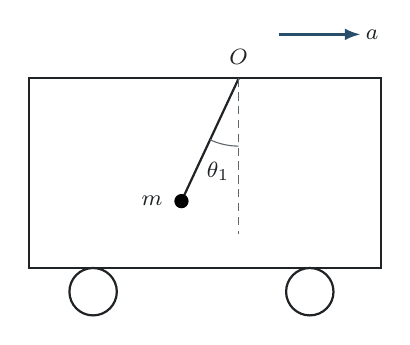
\begin{tikzpicture}[scale=.86]
 \draw[solbody] (-2.7,-1.1) rectangle (2.5,1.7);
 \draw[solbody] (-1.75,-1.45) circle(.35) (1.45,-1.45) circle(.35);
 \coordinate (O) at (.4,1.7); \coordinate (B) at ($(O)+(-115:2)$);
 \draw[solbody] (O)--(B); \fill (B) circle(3pt);
 \node[sollabel,left=5pt] at (B) {$m$};
 \node[sollabel,above=3pt] at (O) {$O$};
 \draw[solgeom] (O)--++(0,-2.3);
 \draw[draw=TextGray] ($(O)+(-90:1)$) arc[start angle=-90,end angle=-115,radius=1];
 \node[sollabel] at ($(O)+(-102.5:1.4)$) {$\theta_1$};
 \draw[solforce] (1,2.35)--(2.2,2.35) node[right,sollabel] {$a$};
\end{tikzpicture}\diagcaption{图 2.24}{车向右匀加速；平衡时细绳与竖直线夹角为 $\theta_1$。}\end{minipage}\end{center}}

\newcommand{\soldiagTwoTwentyFour}{%
\begin{center}\begin{minipage}{\linewidth}\centering\begin{tikzpicture}[scale=.9]
 \node[solpanel] at (-2.4,2.7) {平衡时：三力矢量和为零};
 \fill (-2.4,.4) circle(2pt);
 \draw[solforce] (-2.4,.4)--++(0,-1.5) node[below,sollabel] {$mg$};
 \draw[solforce] (-2.4,.4)--++({-1.5*tan(25)},0) node[left,sollabel] {$ma$};
 \draw[solforce] (-2.4,.4)--++({1.5*tan(25)},1.5) node[above right,sollabel] {$T$};
 \node[solpanel] at (2.3,2.7) {从竖直位置静止释放};
 \coordinate (O) at (3.5,1.9);
 \coordinate (Bz) at ($(O)+(-90:2.6)$);
 \coordinate (Be) at ($(O)+(-115:2.6)$);
 \coordinate (Bt) at ($(O)+(-140:2.6)$);
 \draw[solgeom] (O)--(Bz);
 \draw[solgeom] (O)--(Be);
 \draw[solbody] (O)--(Bt);
 \draw[solgeom] (Bz) arc[start angle=-90,end angle=-140,radius=2.6];
 \foreach \P/\lab/\anc in {Bz/B_0/below right,Be/B_e/below,Bt/B_2/left}{
  \fill (\P) circle(2pt) node[\anc=4pt,sollabel] {$\lab$};
 }
 \node[sollabel,above right=3pt] at (O) {$O$};
 \draw[draw=TextGray] ($(O)+(-90:.72)$) arc[start angle=-90,end angle=-115,radius=.72];
 \node[sollabel] at ($(O)+(-102.5:1.02)$) {$\theta_1$};
 \draw[draw=TextGray] ($(O)+(-90:1.6)$) arc[start angle=-90,end angle=-140,radius=1.6];
 \node[sollabel] at ($(O)+(-122:1.95)$) {$\theta_2$};
 \draw[solforce] (4.65,1.2)--++(-115:1.25) node[right=5pt,sollabel] {$\vec g_{\rm eff}$};
\end{tikzpicture}\diagcaption{解图}{$B_0$ 为释放点，$B_e$ 为平衡点，$B_2$ 为另一端点；$OB_e$ 平行于有效重力，$\theta_2=2\theta_1$。}\end{minipage}\end{center}}

\newcommand{\probdiagTwoTwentyFive}{%
\begin{center}\begin{minipage}{\linewidth}\centering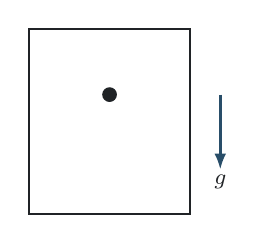
\begin{tikzpicture}[scale=.76]
  \draw[solbody] (-1.35,-1.55) rectangle (1.35,1.55);
  \fill[Ink] (0,.45) circle (3.5pt);
  \draw[solforce] (1.85,.45)--++(0,-1.25) node[below,sollabel] {$g$};
\end{tikzpicture}\diagcaption{图 2.25}{电梯与内部物体同时自由下落。}\end{minipage}\end{center}}

\newcommand{\soldiagTwoTwentyFive}{%
\begin{center}\begin{minipage}{\linewidth}\centering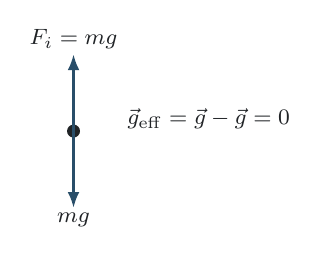
\begin{tikzpicture}[scale=.78]
  \fill[Ink] (0,0) circle (3pt);
  \draw[solforce] (0,0)--++(0,-1.25) node[below,sollabel] {$mg$};
  \draw[solforce] (0,0)--++(0,1.25) node[above,sollabel] {$F_i=mg$};
  \node[sollabel] at (2.2,.2) {$\vec g_{\rm eff}=\vec g-\vec g=0$};
\end{tikzpicture}\diagcaption{解图}{在自由落体电梯系中，惯性力与重力抵消，局部呈现失重。}\end{minipage}\end{center}}

\newcommand{\probdiagTwoTwentySix}{%
\begin{center}\begin{minipage}{\linewidth}\centering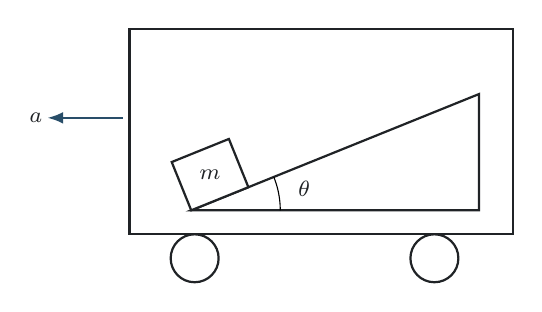
\begin{tikzpicture}[scale=.87]
 \def\th{22}
 \draw[solbody] (-2.8,-1.2) rectangle (2.8,1.8);
 \draw[solbody] (-1.85,-1.55) circle(.35) (1.65,-1.55) circle(.35);
 \coordinate (L) at (-1.9,-.85);
 \coordinate (R) at (2.3,-.85);
 \coordinate (P) at ($(L)+(4.2,{4.2*tan(\th)})$);
 \coordinate (S) at ($(L)+(\th:.45)$);
 \coordinate (B) at ($(S)+({90+\th}:.38)$);
 \draw[solbody] (L)--(R)--(P)--cycle;
 \begin{scope}[shift={(B)},rotate=\th]\draw[solbody,fill=white] (-.45,-.38) rectangle (.45,.38);\end{scope}
 \node[sollabel] at (B) {$m$};
 \draw (L)++(1.3,0) arc[start angle=0,end angle=\th,radius=1.3];
 \node[sollabel] at ($(L)+(11:1.68)$) {$\theta$};
 \draw[solforce] (-2.9,.5)--(-4,.5) node[left,sollabel] {$a$};
\end{tikzpicture}\diagcaption{图 2.26}{汽车向左加速，物块从斜面底端释放；物块底面与斜面贴合。}\end{minipage}\end{center}}

\newcommand{\soldiagTwoTwentySix}{%
\begin{center}\begin{minipage}{\linewidth}\centering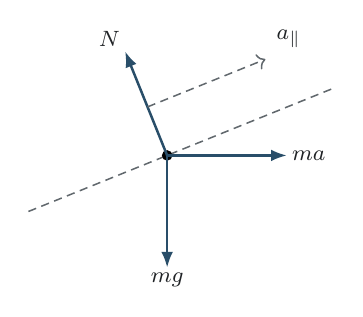
\begin{tikzpicture}[scale=.95]
 \draw[solgeom] (202:2)--(22:2.4);
 \fill (0,0) circle(2pt);
 \draw[solforce] (0,0)--(1.6,0) node[right,sollabel] {$ma$};
 \draw[solforce] (0,0)--(0,-1.5) node[below,sollabel] {$mg$};
 \draw[solforce] (0,0)--(112:1.5) node[above left,sollabel] {$N$};
 \draw[solgeom,->] ($(0,0)+(112:.7)$)--++(22:1.7) node[above right=3pt,sollabel] {$a_{\parallel}$};
\end{tikzpicture}\diagcaption{解图}{$N$ 垂直斜面；沿斜面向上取正，$a_{\parallel}=a\cos\theta-g\sin\theta$。}\end{minipage}\end{center}}

\newcommand{\probdiagTwoTwentySeven}{%
\begin{center}\begin{minipage}{\linewidth}\centering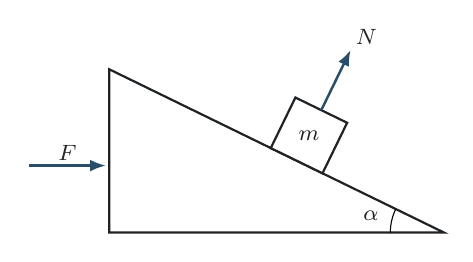
\begin{tikzpicture}[scale=.85]
 \def\al{26}
 \coordinate (L) at (-2.5,-1);
 \coordinate (R) at (2.5,-1);
 \coordinate (P) at ($(L)+(0,{5*tan(\al)})$);
 \coordinate (S) at ($(P)!.56!(R)$);
 \coordinate (B) at ($(S)+({90-\al}:.42)$);
 \draw[solbody] (L)--(R)--(P)--cycle;
 \begin{scope}[shift={(B)},rotate=-\al]\draw[solbody,fill=white] (-.43,-.42) rectangle (.43,.42);\end{scope}
 \node[sollabel] at (B) {$m$};
 \draw[solforce] ($(B)+({90-\al}:.42)$)--++({90-\al}:1) node[above right,sollabel] {$N$};
 \draw (R)++({180-\al}:.8) arc[start angle={180-\al},end angle=180,radius=.8];
 \node[sollabel] at ($(R)+(167:1.12)$) {$\alpha$};
 \draw[solforce] (-3.7,0)--(-2.55,0) node[midway,above,sollabel] {$F$};
\end{tikzpicture}\diagcaption{图 2.27}{水平力推动斜面向右；支持力 $N$ 垂直于接触面。}\end{minipage}\end{center}}

\newcommand{\soldiagTwoTwentySeven}{%
\begin{center}\begin{minipage}{\linewidth}\centering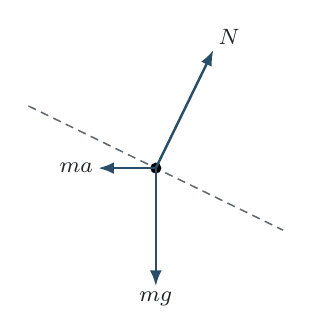
\begin{tikzpicture}[scale=1]
 \draw[solgeom] (154:1.8)--(-26:1.8);
 \fill (0,0) circle(2pt);
 \draw[solforce] (0,0)--(0,-1.5) node[below,sollabel] {$mg$};
 \draw[solforce] (0,0)--({-1.5*tan(26)},0) node[left,sollabel] {$ma$};
 \draw[solforce] (0,0)--({1.5*tan(26)},1.5) node[above right,sollabel] {$N$};
\end{tikzpicture}\diagcaption{解图}{虚线与题图斜面同向；平衡时 $N$ 正好抵消重力和惯性力的合力，并与斜面垂直。}\end{minipage}\end{center}}

\newcommand{\probdiagTwoTwentyEight}{%
\begin{center}\begin{minipage}{\linewidth}\centering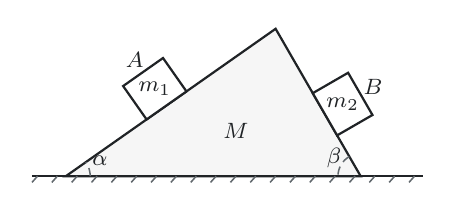
\begin{tikzpicture}[scale=.72]
  % The two slopes deliberately have visibly different inclinations, as in the
  % source figure: alpha is the gentler left slope and beta the steeper right one.
  \coordinate (L) at (-3.05,-1.05);
  \coordinate (P) at (.65,1.55);
  \coordinate (R) at (2.15,-1.05);
  \draw[solbody,fill=SoftGray] (L)--(P)--(R)--cycle;
  \draw[solbody] (-3.65,-1.05)--(3.25,-1.05);
  \foreach \x in {-3.55,-3.20,...,3.15}
    \draw[solgeom] (\x,-1.05)--++(-.16,-.18);

  % Each block is drawn in local slope coordinates; y=0 is its contact face.
  \coordinate (SL) at ($(L)!.48!(P)$);
  \pgfmathsetmacro{\leftang}{atan2(2.6,3.7)}
  \pgfmathsetmacro{\rightang}{-atan2(2.6,1.5)}
  \begin{scope}[shift={(SL)},rotate=\leftang]
    \draw[solbody,fill=white] (-.43,0) rectangle (.43,.72);
    \node[sollabel] at (0,.36) {$m_1$};
    \node[sollabel] at (0,.98) {$A$};
  \end{scope}
  \coordinate (SR) at ($(P)!.58!(R)$);
  \begin{scope}[shift={(SR)},rotate=\rightang]
    \draw[solbody,fill=white] (-.43,0) rectangle (.43,.72);
    \node[sollabel] at (0,.36) {$m_2$};
    \node[sollabel] at (0,.98) {$B$};
  \end{scope}

  \draw[solgeom] ([xshift=.43cm]L) arc[start angle=0,end angle=35.1,radius=.43];
  \draw[solgeom] ([shift={(120:.40)}]R) arc[start angle=120,end angle=180,radius=.40];
  \node[sollabel] at (-2.45,-.78) {$\alpha$};
  \node[sollabel] at (1.68,-.73) {$\beta$};
  \node[sollabel] at (-.05,-.25) {$M$};
\end{tikzpicture}\diagcaption{图 2.28}{双斜面在光滑水平面上自由运动。}\end{minipage}\end{center}}

\newcommand{\soldiagTwoTwentyEight}{%
\begin{center}\begin{minipage}{\linewidth}\centering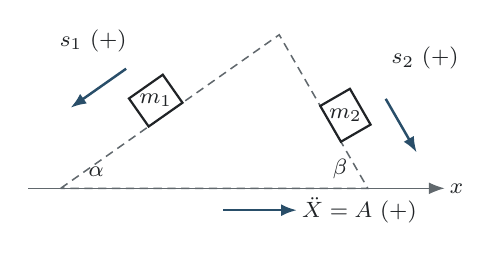
\begin{tikzpicture}[scale=.75]
  \coordinate (L) at (-3.05,-.85);
  \coordinate (P) at (.65,1.75);
  \coordinate (R) at (2.15,-.85);
  \draw[solgeom] (L)--(P)--(R)--cycle;
  \draw[axis] (-3.60,-.85)--(3.45,-.85) node[right,sollabel] {$x$};

  \coordinate (SL) at ($(L)!.48!(P)$);
  \pgfmathsetmacro{\leftang}{atan2(2.6,3.7)}
  \pgfmathsetmacro{\rightang}{-atan2(2.6,1.5)}
  \begin{scope}[shift={(SL)},rotate=\leftang]
    \draw[solbody,fill=white] (-.35,0) rectangle (.35,.58);
    \node[sollabel] at (0,.29) {$m_1$};
    \draw[solforce] (-.10,1.02)--++(-1.15,0);
  \end{scope}
  \coordinate (SR) at ($(P)!.58!(R)$);
  \begin{scope}[shift={(SR)},rotate=\rightang]
    \draw[solbody,fill=white] (-.35,0) rectangle (.35,.58);
    \node[sollabel] at (0,.29) {$m_2$};
    \draw[solforce] (.10,1.02)--++(1.05,0);
  \end{scope}

  \node[sollabel] at (-2.5,1.65) {$s_1\ (+)$};
  \node[sollabel] at (3.12,1.35) {$s_2\ (+)$};
  \draw[solforce] (-.30,-1.22)--++(1.25,0)
    node[right,sollabel] {$\ddot X=A\ (+)$};
  \node[sollabel] at (-2.45,-.57) {$\alpha$};
  \node[sollabel] at (1.68,-.52) {$\beta$};
\end{tikzpicture}\diagcaption{解图}{取 $x$ 轴向右；$s_1,s_2$ 分别沿左右斜面向下为正，斜面加速度 $A=\ddot X$ 向右为正。}\end{minipage}\end{center}}

\newcommand{\probdiagTwoTwentyNine}{%
\begin{center}\begin{minipage}{\linewidth}\centering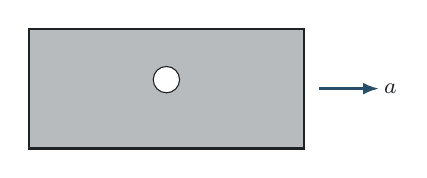
\begin{tikzpicture}[scale=.76]
  \fill[TextGray!45] (-2.3,-1.0) rectangle (2.3,1.0); \draw[solbody] (-2.3,-1.0) rectangle (2.3,1.0);
  \fill[white,draw=Ink] (0,.15) circle (.22);
  \draw[solforce] (2.55,0)--++(1.0,0) node[right,sollabel] {$a$};
\end{tikzpicture}\diagcaption{图 2.29}{装满水的水箱向前加速，水中有气泡。}\end{minipage}\end{center}}

\newcommand{\soldiagTwoTwentyNine}{%
\begin{center}\begin{minipage}{\linewidth}\centering\begin{tikzpicture}[scale=.95]
 \foreach \b in {-.8,0,.8}{\draw[solgeom] (-2.1,{1.68+\b})--(2.1,{-1.68+\b});}
 \fill[white,draw=Ink] (0,0) circle(.14);
 \draw[solforce] (0,0)--(-1.12,-1.4) node[below left=4pt,sollabel] {$\vec g_{\rm eff}=(-a,-g)$};
 \draw[solforce] (0,0)--(1.12,1.4) node[above right=4pt,sollabel] {浮力};
 \node[sollabel,anchor=west] at (2.35,-1.1) {等压线};
 \draw[draw=TextGray] (2.3,-1.2)--(1.9,-1.52);
\end{tikzpicture}\diagcaption{解图}{等压线沿 $(g,-a)$ 方向，与有效重力 $(-a,-g)$ 垂直；压力向左下方增大，浮力指向右上方。}\end{minipage}\end{center}}

% 题图保留杆、转轴、质点与给定量；半径投影及圆轨迹在解图中构造。
\newcommand{\probdiagTwoThirty}{%
\begin{center}\begin{minipage}{\linewidth}\centering\begin{tikzpicture}[scale=.95]
 \def\th{35}
 \coordinate (O) at (0,-1.1);
 \coordinate (P) at ($(O)+({90-\th}:2.6)$);
 \draw[solgeom] (O)--(0,2.6) node[above,sollabel] {转轴};
 \draw[solbody] (O)--++({90-\th}:3.6);
 \fill (O) circle(1.5pt) node[below left,sollabel] {$O$};
 \fill (P) circle(2.5pt) node[right=4pt,sollabel] {$P$};
 \draw[draw=TextGray] ($(O)+(0,.65)$) arc[start angle=90,end angle={90-\th},radius=.65];
 \node[sollabel] at ($(O)+(72.5:.94)$) {$\theta$};
 \draw[<->,draw=TextGray] ($(O)+(-35:.4)$)--($(P)+(-35:.4)$) node[midway,below right=4pt,sollabel] {$l$};
 \draw[->,draw=TextGray] (-.65,2.1) arc[start angle=180,end angle=350,x radius=.65,y radius=.17];
 \node[sollabel] at (.9,2.2) {$\omega$};
\end{tikzpicture}\diagcaption{图 2.30}{质点在杆上距固定端 $O$ 为 $l$ 处，杆与竖直转轴夹角为 $\theta$。}\end{minipage}\end{center}}


\newcommand{\soldiagTwoThirtyGeometry}{%
\begin{center}\begin{minipage}{\linewidth}\centering\begin{tikzpicture}[scale=.95]
 \def\th{35}
 \coordinate (O) at (0,-1.1);
 \coordinate (P) at ($(O)+({90-\th}:2.6)$);
 \coordinate (H) at (O |- P);
 \pgfmathsetmacro{\rad}{2.6*sin(\th)}
 \draw[solgeom] ($(H)+(-\rad,0)$) arc[start angle=180,end angle=0,x radius=\rad,y radius=.3];
 \draw[solbody] ($(H)+(-\rad,0)$) arc[start angle=180,end angle=360,x radius=\rad,y radius=.3];
 \draw[solgeom] (O)--(0,2.6) node[above,sollabel] {转轴};
 \draw[solbody] (O)--++({90-\th}:3.6);
 \fill (O) circle(1.5pt) node[below left,sollabel] {$O$};
 \fill (P) circle(2.5pt) node[right=4pt,sollabel] {$P$};
 \draw[solgeom] (H)--(P) node[midway,above=5pt,sollabel] {$r$};
 \draw[draw=TextGray] ($(O)+(0,.65)$) arc[start angle=90,end angle={90-\th},radius=.65];
 \node[sollabel] at ($(O)+(72.5:.94)$) {$\theta$};
 \draw[<->,draw=TextGray] ($(O)+(-35:.4)$)--($(P)+(-35:.4)$) node[midway,below right=4pt,sollabel] {$l$};
 \draw[->,draw=TextGray] (-.65,2.1) arc[start angle=180,end angle=350,x radius=.65,y radius=.17];
 \node[sollabel] at (.9,2.2) {$\omega$};
\end{tikzpicture}\diagcaption{解图}{$OP=l$，水平转动半径 $r=l\sin\theta$；圆轨道后半部以虚线表示。}\end{minipage}\end{center}}

\newcommand{\soldiagTwoThirty}{%
\begin{center}\begin{minipage}{\linewidth}\centering\begin{tikzpicture}[scale=.95]
 \node[solpanel] at (-2.3,2.3) {旋转系中的受力};
 \coordinate (P) at (-2.3,0);
 \draw[solgeom] ($(P)+(235:1.8)$)--($(P)+(55:1.8)$);
 \fill (P) circle(2pt);
 \draw[solforce] (P)--++(1.5,0) node[right,sollabel] {$F_{\rm cf}$};
 \draw[solforce] (P)--++(0,-1.5) node[below,sollabel] {$mg$};
 \draw[solforce] (P)--++(145:1.35) node[above left,sollabel] {$N$};
 \draw[<->,draw=TextGray] ($(P)+(-35:.8)+(235:.4)$)--++(55:.8) node[midway,below right=6pt,sollabel] {$f_s$};
 \node[solpanel] at (2.9,2.3) {沿杆方向的投影};
 \coordinate (Q) at (2.9,0);
 \draw[solgeom] ($(Q)+(235:1.9)$)--($(Q)+(55:1.9)$);
 \fill (Q) circle(2pt);
 \draw[solforce] (Q)--++(55:1.3) node[pos=.65,right=8pt,sollabel] {$F_{{\rm cf},\parallel}$};
 \draw[solforce] (Q)--++(235:1.3) node[pos=.7,below right=7pt,sollabel] {$mg\cos\theta$};
\end{tikzpicture}\diagcaption{解图}{两图的杆方向相同；$N$ 垂直杆，$F_{{\rm cf},\parallel}=m\omega^2l\sin^2\theta$，$f_s$ 沿杆方向并可取正或负。}\end{minipage}\end{center}}

\newcommand{\soldiagTwoThirtyOne}{%
\begin{center}\begin{minipage}{\linewidth}\centering\begin{tikzpicture}[scale=.86]
  \draw[solbody] (0,0) circle (2.05);
  \fill[Ink] (0,0) circle (1.5pt) node[below left=3pt,sollabel] {转轴};
  \fill[DeepBlue] (2.05,0) circle (3.5pt) node[right=5pt,sollabel] {实验对象};
  \draw[solgeom] (0,0)--(2.05,0)
    node[pos=.48,below=4pt,sollabel] {$r=7\,\mathrm m$};
  \draw[solforce] (2.05,0)--(.62,0)
    node[pos=.58,above=4pt,sollabel] {$a_c=5g$};
  \draw[solgeom,-{Latex[length=1.7mm]}] (2.05,0)--++(0,1.05)
    node[above=3pt,sollabel] {$v$};
\end{tikzpicture}\diagcaption{解图}{离心机提供大小为 $5g$ 的水平向心加速度。}\end{minipage}\end{center}}


\begin{document}
\pagenumbering{arabic}
\setcounter{page}{1}
\setcounter{chapter}{2}
\setcounter{section}{2}

\section{非惯性系与惯性力}
\setcounter{equation}{0}

前面曾多次强调，牛顿定律只在惯性参考系中成立。于是自然会产生一个问题：相对于惯性系
做加速运动的非惯性参考系中，物体的运动是否就不能用类似的方式描述？严格地说，牛顿
定律不能直接用于非惯性系；但这并不妨碍我们先在惯性系中写出运动方程，再利用已知的
坐标变换，把它改写成相对于非惯性系的形式。这样做既保留了牛顿定律的适用条件，也能
方便地研究车厢、电梯和转盘中的运动。

考虑两个相对运动的参考系 $S$ 和 $S'$。其中 $S$ 是惯性参考系，$S'$ 相对于 $S$ 以
加速度 $\vec a_r$ 作平动。质量为 $m$ 的质点受到真实合力 $\vec F$，相对于 $S$ 的加速度
为 $\vec a$，相对于 $S'$ 的加速度为
\[
 \vec a'=\vec a-\vec a_r.
\]
由 $\vec F=m\vec a$ 得
\[
 m\vec a'=\vec F-m\vec a_r.
\]
因此，如果希望在 $S'$ 中仍采用“质量乘加速度等于力之和”的形式，就要引入惯性力
\begin{equation}
 \boxed{\vec F_i=-m\vec a_r}. \tag{2.12}
\end{equation}
惯性力是参考系加速带来的表观力，没有施力物体，牛顿第三定律不适用于它。对于相对
非惯性系静止的物体，引入惯性力后，动力学问题常可转化为静力平衡问题。

上述结论并不限于单个质点。若非惯性系中有多个彼此作用的质点，就对每个质量为 $m_i$
的质点同时加入 $-m_i\vec a_r$。真实外力和质点间相互作用力仍按通常方式列出，惯性力
只负责补偿参考系的加速运动。于是每个质点都满足
\[
 m_i\vec a_i'=\vec F_{\mathrm{real},i}+\vec F_{\mathrm{inert},i},
 \qquad \vec F_{\mathrm{inert},i}=-m_i\vec a_r.
\]
这里 $\vec F_{\mathrm{real},i}$ 是第 $i$ 个质点所受真实合力，与惯性力分开记号。
由于所有质点所加惯性力都与各自质量成正比，许多相对车厢或电梯保持静止的问题便可按
平衡问题处理；但必须记住，这只是非惯性坐标中的等效写法，并没有产生新的相互作用。

\subsubsection*{平动非惯性系与等效重力场}

设参考系 $S'$ 相对惯性系作平动，原点加速度为 $\vec a_0$。若两系坐标轴不转动，则
$\vec a=\vec a'+\vec a_0$，于是
\begin{equation}
 m\vec a'=\sum\vec F-m\vec a_0.
\end{equation}
把 $-m\vec a_0$ 称为惯性力，便可在车厢、电梯等非惯性系中沿用平衡和动力学方程。惯性力
与质量成正比，没有施力物体，也没有第三定律的反作用力；它只是坐标系加速在运动方程中的
表现。若所有真实物体都同时受均匀重力 $m\vec g$，可把两者合并为
\begin{equation}
 \vec g_{\rm eff}=\vec g-\vec a_0.
\end{equation}
悬线、自由液面和小振动平衡位置都由有效重力方向决定。

这种局部等效有明确限度。自由落体电梯中，均匀重力与惯性力相消，舱内物体近似失重；但地球
重力随位置改变，不同点的自由落体加速度略有差异，仍会出现潮汐效应。因此自由落体系只能在
足够小的空间和足够短的时间内近似消除均匀重力对自由物体相对运动的影响。
按牛顿力学的定义，它仍是相对地面加速的非惯性系，不能仅因自由物体相对匀速就改变这个判定。
广义相对论中自由落体与局部惯性坐标的联系属于另一理论层次，这里不把两种定义混用。
判断均匀场近似是否可用，应比较被忽略的差异加速度与题目
要求的精度，而不能仅凭“物体正在自由下落”下结论。

若参考系还在转动，需要区分相对位置和绝对位置。设地面惯性系为 $S$，转动系为 $S'$，
$S'$ 原点的位置、速度、加速度分别为 $\vec R_0,\vec V_0,\vec a_0$；
$\vec r$ 是从 $S'$ 原点指向质点的位置矢量，$\vec v'$、$\vec a'$ 是在 $S'$ 中求得的相对速度、相对加速度。
转动系角速度为 $\vec\omega$，角加速度为 $\dot{\vec\omega}$。
对任意矢量 $\vec b$，两种求导满足
\[
 \left(\frac{\dd\vec b}{\dd t}\right)_S
 =\left(\frac{\dd\vec b}{\dd t}\right)_{S'}+\vec\omega\times\vec b.
\]
由绝对位置 $\vec R_0+\vec r$ 求导，得
\[
 \vec v=\vec V_0+\vec v'+\vec\omega\times\vec r.
\]
再求一次导数：$\vec v'$ 产生 $\vec a'+\vec\omega\times\vec v'$，而最后一项产生
$\dot{\vec\omega}\times\vec r+\vec\omega\times(\vec v'+\vec\omega\times\vec r)$。
两处相同的交叉项相加，得到
\begin{equation}
 \vec a=\vec a_0+\vec a'+2\vec\omega\times\vec v'
 +\vec\omega\times(\vec\omega\times\vec r)
 +\dot{\vec\omega}\times\vec r.
\end{equation}
五项依次为原点平动加速度、相对加速度、科里奥利项、随转动产生的向心项和角加速度项。
将除 $\vec a'$ 外的参考系运动项移到动力学方程右侧并乘 $-m$，就得到相应惯性力。
其中 $-m\vec\omega\times(\vec\omega\times\vec r)$ 指向远离转轴的方向，即离心力。
本节转杆问题中原点固定、$\vec\omega$ 恒定且质点相对杆静止，因而
$\vec a_0=0$、$\dot{\vec\omega}=0$、$\vec v'=0$，只需加入离心力。
转盘上运动物体的侧向偏转则还涉及科里奥利项，不能把所有非惯性效应都写成同一个 $-m\vec a_0$。


\begin{origexamplebox}{例 2.24}
很多时候可以近似认为地球表面是一个惯性参考系。现有一辆相对于地面以加速度 $a$ 作
匀加速直线运动的车，车内一个质量为 $m$ 的小球被悬挂在车顶。求小球相对车厢静止时，
悬线与竖直方向的夹角 $\theta_1$。悬线长为 $l$，轻且不可伸长；若将小球拉到竖直方向，
相对车厢由静止释放，求另一侧最高点与竖直方向的夹角 $\theta_2$。
全过程中车的加速度保持不变，忽略阻力及小球与车厢边界的碰撞。
\probdiagTwoTwentyFour
\end{origexamplebox}

\Needspace{16\baselineskip}
\begin{xesolution}
以车为参考系。车向右加速，因此小球受到大小为 $ma$、方向向左的惯性力。平衡位置的
受力和有效重力方向如解图所示：
\soldiagTwoTwentyFour
由水平、竖直方向平衡条件
\[
 T\sin\theta_1=ma,
 \qquad
 T\cos\theta_1=mg,
\]
得到
\[
 \boxed{\tan\theta_1=\frac ag}.
\]
有效重力大小为 $g_{\rm eff}=\sqrt{g^2+a^2}$，方向相对竖直向后偏 $\theta_1$。
图中 $B_0$ 是竖直释放点，$B_e$ 是平衡位置，$B_2$ 是另一转折点。设摆线相对通常竖直方向
向后偏转的角度为 $\theta$，它与有效重力的夹角为 $\theta-\theta_1$。
沿有效重力方向向下的坐标为 $l\cos(\theta-\theta_1)$，因此以悬点为势能零点，
与恒定有效重力对应的势能是
\[
 U=-mg_{\rm eff}l\cos(\theta-\theta_1).
\]
这是将重力和恒定惯性力共同计入的有效势能。车系中绳张力始终与相对速度垂直，不做功，
故小球相对车厢的动能 $mv'^2/2$ 与这一势能之和保持不变。
小球从 $\theta=0$ 处静止释放。另一侧最高点也是速度为零，能量守恒给出
\[
 \cos(\theta_2-\theta_1)=\cos\theta_1.
\]
除初始点外的另一个转折点为
\[
 \boxed{\theta_2=2\theta_1
 =2\arctan\frac ag}.
\]
图中这两个转折位置关于 $OB_e$ 对称，但并不关于通常的竖直线对称。
在摆动范围内张力为 $ml^{-1}v'^2+mg_{\rm eff}\cos(\theta-\theta_1)\ge mg>0$，
所以悬线保持绷紧。$a\to0$ 时两个角均趋于零，竖直释放的小球不再偏摆。
\end{xesolution}

\begin{origexamplebox}{例 2.25}
不计空气阻力，证明在地表附近自由下落的“电梯”中，仅受重力、彼此不相互作用且尚未碰壁的
自由物体相对于电梯均保持静止或作匀速直线运动。思考一下：在证明过程中忽略了什么，
得到了什么样的结论？这个电梯是一个惯性
参考系吗？
\probdiagTwoTwentyFive
\end{origexamplebox}

\begin{xesolution}
在地面惯性系的近似下，电梯与其中任意自由物体都只受重力，因而
\[
 \vec a_{\rm E}=\vec g,
 \qquad
 \vec a_{\rm P}=\vec g.
\]
故物体相对电梯的加速度为
\[
 \vec a_{\rm rel}=\vec a_{\rm P}-\vec a_{\rm E}=0.
\]
于是它相对电梯保持静止或作匀速直线运动。在电梯系中也可以用解图理解：向上的惯性力
$-m\vec g$ 恰好抵消向下的重力 $m\vec g$。
\soldiagTwoTwentyFive
这里忽略了地球自转、空气阻力以及重力随高度和水平位置的变化。尤其是重力场不完全均匀：
相距有限的物体具有微小的相对加速度，即潮汐效应。

在牛顿力学中，这个电梯相对于地面惯性系有加速度，因此不是惯性参考系；只是对足够小的
空间和足够短的时间，均匀重力与惯性力抵消，使自由物体呈现相对匀速的运动。这个结论也是
失重现象与等效原理的经典出发点。
\end{xesolution}

\begin{origexamplebox}{例 2.26}
如图所示，汽车内固定有一个倾角为 $\theta$ 的斜面，斜面表面光滑，底部有一个质量为
$m$ 的小物块。开始时系统静止，某时刻汽车突然开始向左以加速度 $a$ 作匀加速运动。
求使物块刚好具有沿斜面向上运动趋势的临界加速度；若要求物块从静止开始真正向上滑动，
$a$ 还应满足什么条件？
\probdiagTwoTwentySix
\end{origexamplebox}

\begin{xesolution}
在汽车参考系中，惯性力 $ma$ 水平向右。沿斜面方向分解重力与惯性力，受力关系如解图：
\soldiagTwoTwentySix
取沿斜面向上为正，则
\[
 ma_{\parallel}=ma\cos\theta-mg\sin\theta.
\]
使物块刚好具有向上运动趋势的临界条件为 $a_{\parallel}=0$，故
\[
 \boxed{a_{\min}=g\tan\theta}.
\]
在临界值处沿斜面合力为零，物块不会从静止状态自行上滑；若要真正开始向上运动，必须有
\[
 \boxed{a>g\tan\theta}.
\]
\end{xesolution}

\begin{origexamplebox}{例 2.27}
如图所示，在光滑水平面上有一光滑斜面，倾角为 $\alpha$。一质量为 $m$ 的物体放在斜面上，
在水平力 $F$ 推动下恰使物体 $m$ 与斜面无相对滑动。求斜面对物块弹力的大小。
\probdiagTwoTwentySeven
\end{origexamplebox}

\begin{xesolution}
以随斜面向右加速的参考系分析。物块相对斜面静止，受到重力、支持力和水平向左的惯性力，
三力平衡，如解图所示：
\soldiagTwoTwentySeven
沿斜面方向平衡要求
\[
 ma\cos\alpha=mg\sin\alpha,
 \qquad\Rightarrow\qquad a=g\tan\alpha.
\]
沿斜面法向平衡，或者直接在地面惯性系的竖直方向列式，得到
\[
 N\cos\alpha=mg.
\]
因此
\[
 \boxed{N=\frac{mg}{\cos\alpha}}.
\]
题设没有给出斜面质量，所以不能由现有条件求 $F$；但弹力由物块的竖直平衡唯一确定，
不需要知道 $F$ 和斜面质量。
\end{xesolution}

\begin{origexamplebox}{例 2.28}
如图所示，一个质量为 $M$、两边倾角分别为 $\alpha$ 和 $\beta$ 的斜面放在水平面上。
两个斜面上分别放有质量为 $m_1$ 和 $m_2$ 的物块 $A$ 和 $B$。忽略一切摩擦，求由静止
释放后所有物体的加速度。
\probdiagTwoTwentyEight
\end{origexamplebox}

\begin{xesolution}
取水平向右为正，设斜面的水平加速度为 $A=\ddot X$；令 $s_1,s_2$ 分别表示两物块相对
斜面沿各自斜面向下的位移。坐标和正方向如解图：
\soldiagTwoTwentyEight
地面系中的坐标关系为（省略不影响加速度的坐标常数）
\[
 x_1=X-s_1\cos\alpha,\quad y_1=-s_1\sin\alpha,
 \qquad x_2=X+s_2\cos\beta,\quad y_2=-s_2\sin\beta.
\]
两块分别受重力和垂直于各自斜面的支持力。以左块为例，将加速度沿左斜面向下投影，得到
\[
 (A-\ddot s_1\cos\alpha)(-\cos\alpha)
 +(-\ddot s_1\sin\alpha)(-\sin\alpha)
 =\ddot s_1-A\cos\alpha.
\]
支持力投影为零，重力投影为 $m_1g\sin\alpha$。右块同理，两个方程为
\[
 \ddot s_1-A\cos\alpha=g\sin\alpha,
 \qquad
 \ddot s_2+A\cos\beta=g\sin\beta.
\]
系统水平方向不受外力，因此
\[
 (M+m_1+m_2)A-m_1\ddot s_1\cos\alpha
 +m_2\ddot s_2\cos\beta=0.
\]
记
\[
 D=M+m_1\sin^2\alpha+m_2\sin^2\beta.
\]
联立解得斜面的加速度
\[
 \boxed{A=\frac{g\left(m_1\sin\alpha\cos\alpha
 -m_2\sin\beta\cos\beta\right)}{D}}.
\]
$A>0$ 表示斜面向右，$A<0$ 表示向左。两物块相对斜面的加速度分别为
\[
 \boxed{a_{1/\!M}=\ddot s_1=g\sin\alpha+A\cos\alpha},
\]
\[
 \boxed{a_{2/\!M}=\ddot s_2=g\sin\beta-A\cos\beta}.
\]
它们相对地面的加速度分量为
\[
 \boxed{
 a_{1x}=A-\ddot s_1\cos\alpha,
 \qquad
 a_{1y}=-\ddot s_1\sin\alpha},
\]
\[
 \boxed{
 a_{2x}=A+\ddot s_2\cos\beta,
 \qquad
 a_{2y}=-\ddot s_2\sin\beta}.
\]
这些式子给出了斜面和两个物块的全部对地加速度。
若 $m_1=m_2$ 且 $\alpha=\beta$，分子相消，$A=0$，两块沿固定斜面以 $g\sin\alpha$ 下滑。
若 $m_2\to0$，公式还原为单物块在活动斜面上的结果。两个法向力分别为
$N_1=m_1(g\cos\alpha-A\sin\alpha)$、$N_2=m_2(g\cos\beta+A\sin\beta)$。
例如代入后
\[
 N_1=\frac{m_1g[M\cos\alpha+m_2\sin\beta\sin(\alpha+\beta)]}{D}>0,
\]
$N_2$ 交换下标及角度可得同样结论，因此在 $M>0$、两倾角均为锐角时接触约束成立。
\end{xesolution}

\begin{origexamplebox}{例 2.29}
一个装满水的水箱中有一个气泡。当水箱以加速度 $a$ 向前加速运动时，这个气泡将
\underline{\hspace{3em}}（向前、向后）运动。
\probdiagTwoTwentyNine
\end{origexamplebox}

\begin{xesolution}
在水箱参考系中，液体受到向后的惯性力。把重力和惯性力合成，有效重力方向为“向下且
向后”。取 $x$ 向前、$y$ 向上，则 $\vec g_{\rm eff}=(-a,-g)$。
在液体随箱共同加速、相对流动的瞬态可忽略时，取宽 $\dd x$、横截面积 $S$ 的液体微元，
水平平衡要求 $-S\dd p-\rho S\dd x\,a=0$，即 $\partial p/\partial x=-\rho a$。
竖直方向同理有 $\partial p/\partial y=-\rho g$。所以
\[
 p=p_0-\rho ax-\rho gy.
\]
压强沿有效重力方向增大；在等压线上 $a\dd x+g\dd y=0$，故其斜率为 $-a/g$，
与有效重力垂直。图中箭头及等压线体现了这一关系：
\soldiagTwoTwentyNine
体积为 $V$ 的气泡受到周围水的合压力
$\vec F_b=-\rho_{\text{水}}V\vec g_{\rm eff}$；再加上气泡自身的重力和惯性力，
驱动力为 $(\rho_{\text{气}}-\rho_{\text{水}})V\vec g_{\rm eff}$。
气泡密度远小于水，所以它相对水箱向上且向前运动。这里只判断运动趋势，
实际加速度和速度还受周围液体运动及阻力影响。横向选择应填
\[
 \boxed{\text{向前}}.
\]
容易混淆之处是：致密小物体趋向有效重力方向，轻气泡却因浮力而向相反方向运动。
\end{xesolution}

如果物体相对于匀速转动的参考系保持静止，那么在惯性系中它作匀速圆周运动，所需合力指向转轴，大小为
\begin{equation}
 F=m\omega^2r \tag{2.13}
\end{equation}
在转动系看来，可引入大小相同、方向沿径向向外的离心力，使相对
静止问题写成平衡形式。

\begin{origexamplebox}{例 2.30}
一根细杆与竖直方向的夹角为 $0<\theta<\pi/2$，绕通过其固定下端 $O$ 的竖直轴，
以恒定角速度 $\omega\ge0$ 匀速转动。杆上距 $O$ 为 $l>0$ 处套有一个质点。
先设接触无摩擦，质点能够与杆保持相对静止，求角速度
$\omega$。如果质点与杆之间有摩擦，且最大静摩擦因数为 $\mu$，求能够保持相对静止的角速度
$\omega$ 的范围。
\probdiagTwoThirty
\end{origexamplebox}

\begin{xesolution}
先作质点到竖直转轴的水平投影。杆长段 $OP=l$ 与竖直方向成 $\theta$，故转动半径为 $r=l\sin\theta$：
\soldiagTwoThirtyGeometry
在随杆转动的参考系中，质点相对静止，受到
重力、杆的支持力以及水平向外的离心力
\[
 F_{\rm cf}=m\omega^2l\sin\theta.
\]
沿杆方向的两个分量如解图所示：
\soldiagTwoThirty
无摩擦时沿杆方向平衡：
\[
 m\omega^2l\sin^2\theta=mg\cos\theta.
\]
因此
\[
 \boxed{\omega=\sqrt{\frac{g\cos\theta}{l\sin^2\theta}}}.
\]

有摩擦时，维持平衡所需摩擦力的大小为
\[
 |f|=m\left|g\cos\theta-\omega^2l\sin^2\theta\right|.
\]
重力与离心力在垂直于杆方向的合分量由支持力平衡，故
\[
 N=m\sin\theta\left(g+\omega^2l\cos\theta\right).
\]
静摩擦条件 $|f|\le\mu N$ 给出最稳妥的角速度范围表达式
\[
 \boxed{
 \left|g\cos\theta-\omega^2l\sin^2\theta\right|
 \le\mu\sin\theta\left(g+\omega^2l\cos\theta\right)}.
\]
取沿杆离开 $O$ 为正，所需有符号摩擦力为
$f_s=m(g\cos\theta-\omega^2l\sin^2\theta)$：转得慢时它阻止下滑，沿杆向上；
转得快时它阻止外滑，沿杆向下。拆开绝对值并令 $z=\omega^2\ge0$，得到
\begin{align*}
 zl(\sin^2\theta+\mu\sin\theta\cos\theta)&\ge g(\cos\theta-\mu\sin\theta),\\
 zl(\sin^2\theta-\mu\sin\theta\cos\theta)&\le g(\cos\theta+\mu\sin\theta).
\end{align*}
第一式中 $z$ 的系数总为正，因而对任何 $\mu\ge0$ 都给出下界
\[
 \boxed{\omega^2\ge
 \max\!\left\{0,
 \frac{g(\cos\theta-\mu\sin\theta)}
 {l(\sin^2\theta+\mu\sin\theta\cos\theta)}\right\}},
\]
第二式右端为正。若 $\mu<\tan\theta$，左端系数也为正，另有上界
\[
 \boxed{\omega^2\le
 \frac{g(\cos\theta+\mu\sin\theta)}
 {l(\sin^2\theta-\mu\sin\theta\cos\theta)}}.
\]
当 $\mu=\tan\theta$ 时第二式左端为零；当 $\mu>\tan\theta$ 时其左端非正。
两种情况都自动满足第二式，所以只需满足前述下界，理想模型下\textbf{没有有限的角速度上界}。
若 $\mu=0$，上下界重合为无摩擦结果；若 $\mu\ge\cot\theta$，下界为零，说明静止杆上也能靠摩擦托住质点。
\end{xesolution}

\clearpage
\begin{origexamplebox}{例 2.31}
航空医学研究中使用的离心机，是一个绕竖直轴转动的水平杆，杆的一端携带一个实验对象。
如果从转动中心到实验对象的距离为 $7\,\mathrm m$，离心机要转动多快，才能使乘坐者获得
大小为 $5g$ 的水平向心加速度？
\end{origexamplebox}

\begin{xesolution}
离心机提供的水平向心加速度满足
\[
 \omega^2r=5g.
\]
运动关系如解图所示：
\soldiagTwoThirtyOne
取 $r=7\,\mathrm m$、$g=9.8\,\mathrm{m/s^2}$，得
\[
 \boxed{\omega=\sqrt{\frac{5g}{r}}=\sqrt7
 \approx2.65\,\mathrm{rad/s}}.
\]
对应转动频率和转速为
\[
 f=\frac{\omega}{2\pi}\approx0.421\,\mathrm{Hz},
 \qquad
 \boxed{n\approx25.3\,\mathrm{r/min}},
\]
周期约为 $2.37\,\mathrm s$。

如果实际装置把“$5g$ 过载”定义为座椅支持力对应的总表观加速度，并计入竖直重力，条件将
改为
\[
 \sqrt{(\omega^2r)^2+g^2}=5g.
\]
这与题设明确给出的“水平向心加速度为 $5g$”是两个不同的指标。
\end{xesolution}

\end{document}
